\chapter{Benchmark-I}

\section{The Task}
The objective of the program is simple. It generates an array up to a certain length of integers. It then computes the square roots of these, saving them to another array of the same length. This operation it performs on both the CPU and the GPU, and reports the process times taken on the two and their ratio. These three numbers are measured for a range of process size (total number of operations required for the process).
Therefore, with the array size fixed, the task is instead repeated, i.e. square roots of the same first array are computed and repeatedly saved to the second array, replacing the identical values before. In terms of utility this operation is an unproductive repetition, but in terms of analysing optimization, which is our goal, this serves equally well as any other, more utilitarian method of lengthening the process. In fact, increasing the array size would have meant computing square roots of increasingly larger numbers, which is not a proportional
increase in task size. However, repeating the same computation is a linear way to increase the task size, and thus the results may conveniently be plotted on a linear scale. The repetition loop is lengthened in steps of 100. For each length of the loop, process times on the GPU, CPU and their ratio are measured for 10 samples, and the average of each is written to a file.

\section{Code Walkthrough}
Code Walkthrough mentioned in file codewalkthrough.

\section{Results}

\subsection{Output}
The program displays information from each sample on screen, but writes only the statistics from each sampling to file, without information from all the samples. The first allows easy debugging, while the second allows easy analysis and plotting of the final data.\\\\
The Outputs have been mentioned in the following files :\\\\
\begin{enumerate}
\item samplevsgpu for GPU Result
\item samplevscpu for CPU Result
\item samplevsratio for GPU-CPU Ratio
\item time.txt for Time
\end{enumerate}

\subsection{Plots}
\vspace{1cm}
\textbf{CPU Process Times}\\\\
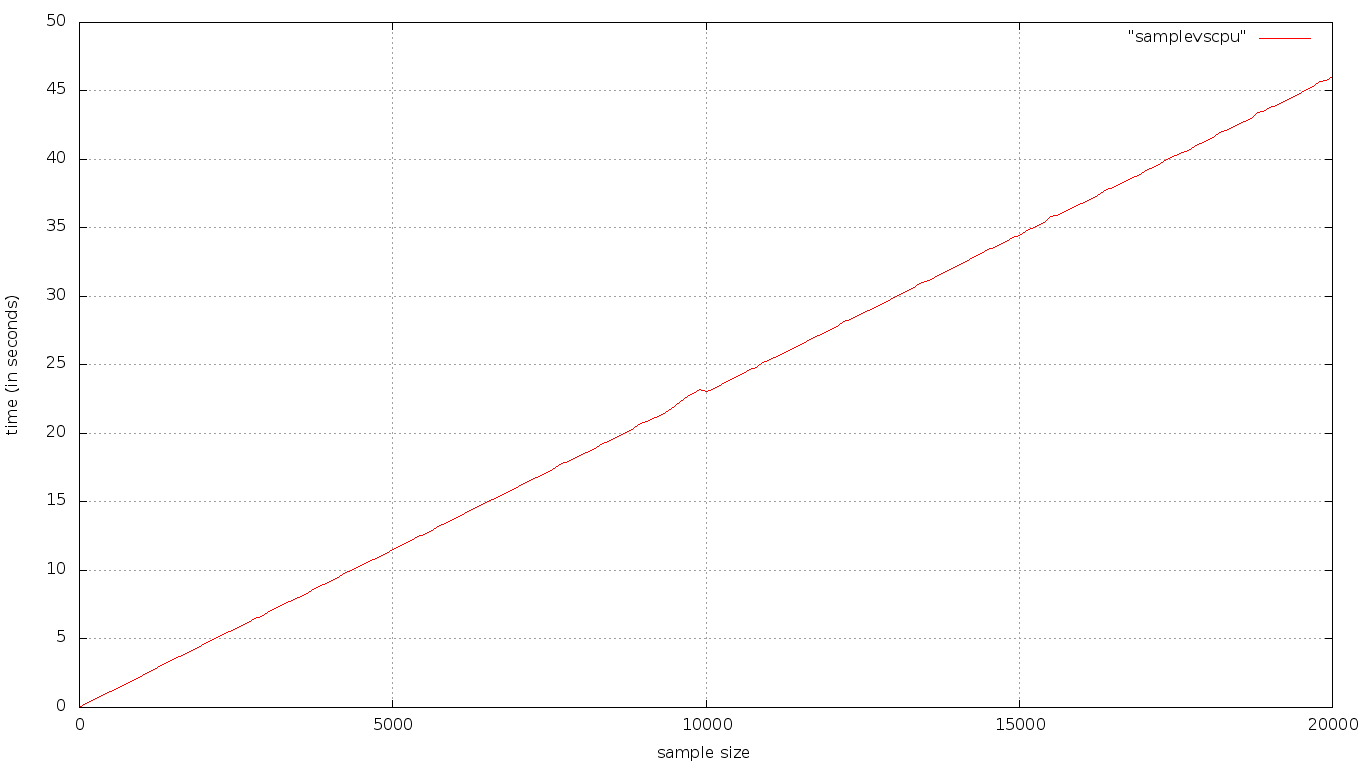
\includegraphics [width=1.2\textwidth]{cpu.png}
\newpage
\textbf{GPU Process Times}\\\\
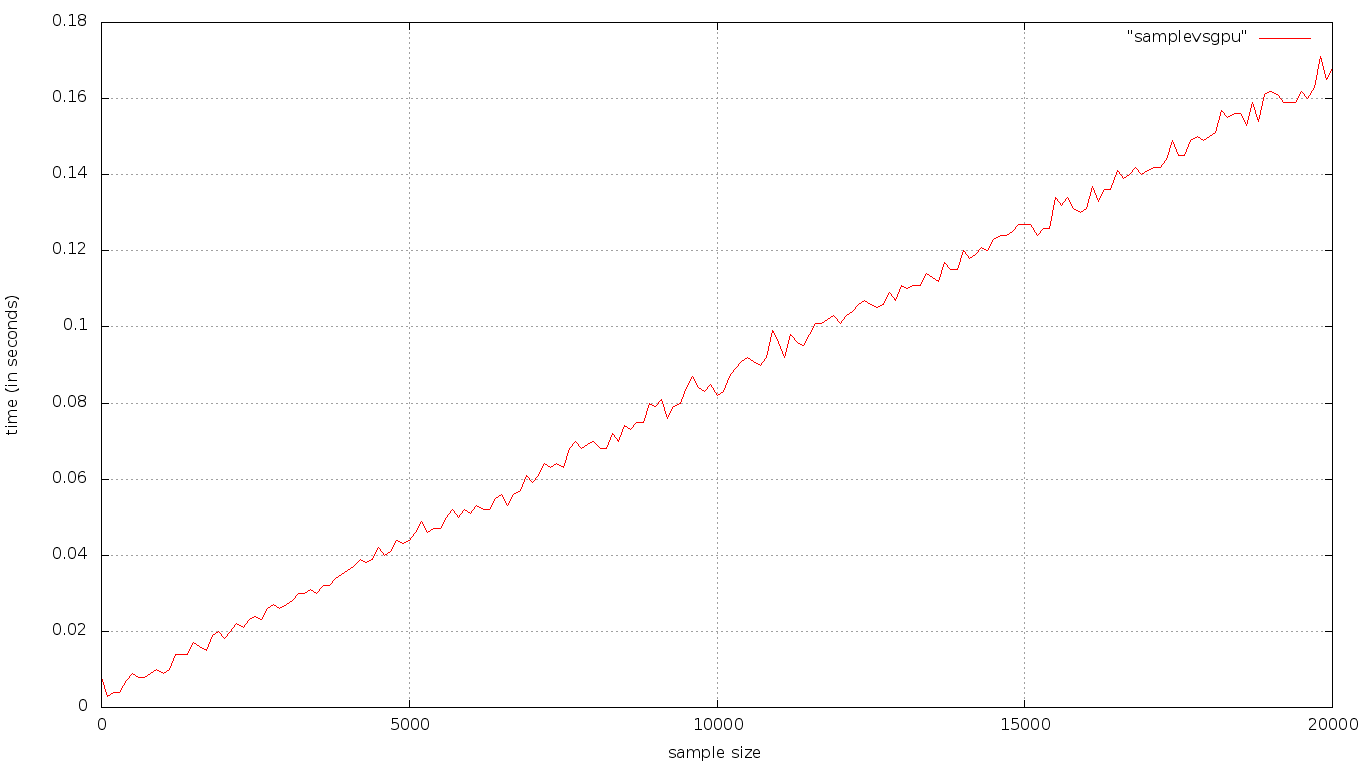
\includegraphics [width=1.2\textwidth]{gpu.png}
\textbf{CPU / GPU Ratio}\\\\
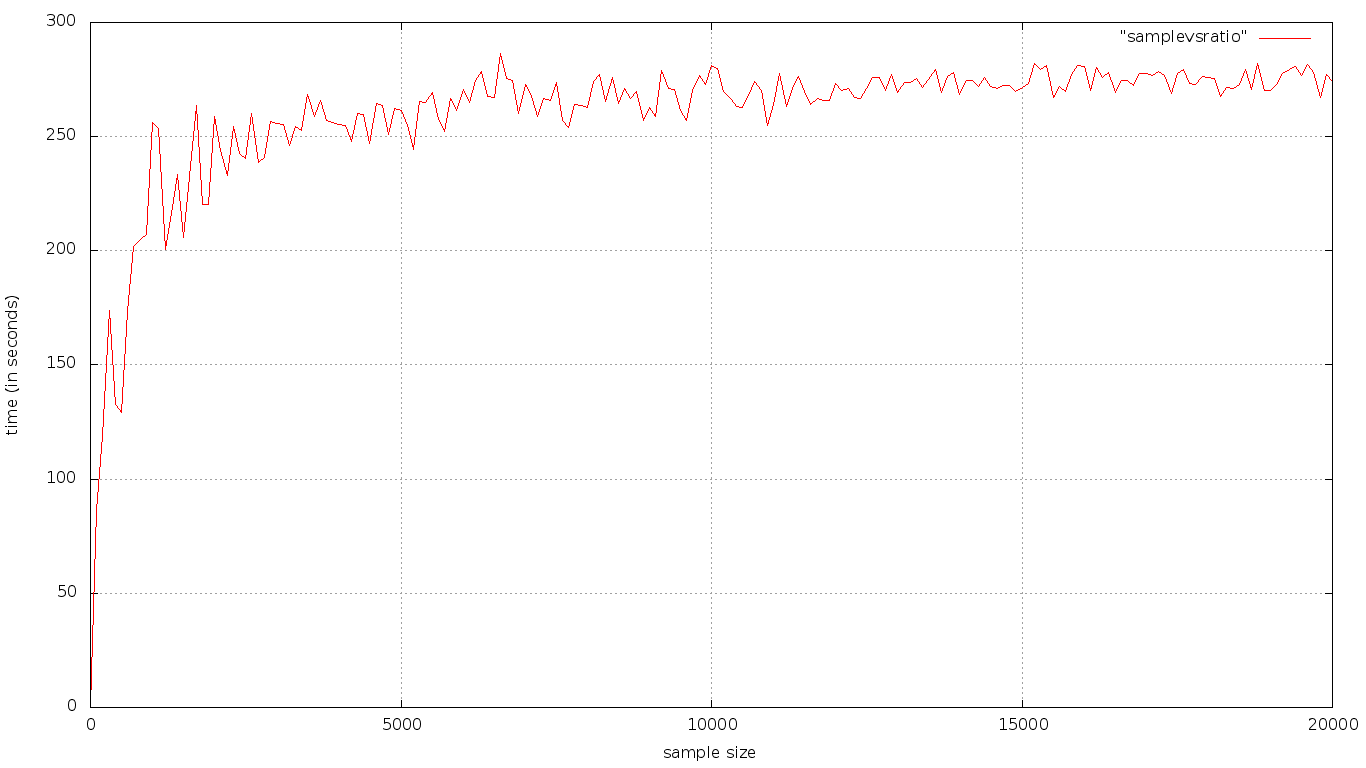
\includegraphics [width=1.2\textwidth]{ratio.png}

\section{Inferences}
\begin{enumerate}
\item For smaller tasks, the GPU is not much faster than the CPU as the data transfer overhead between host and device costs more than time saved by parallelization.
\item The ratio between GPU and CPU speeds, however, does not keep rising with increasing task size. It reaches an asymptote of about a 280-fold efficiency. This occurs when the transfer overheads take negligible time compared to that taken by the actual arithmetical computations on the device.
\item The above code follows \href{http://en.wikipedia.org/wiki/Amdahl's_law}{Amdahl's Law} The speedup of a program using multiple processors in parallel computing is limited by the sequential fraction of the program. For example, if 95\% of the program can be parallelized, the theoretical maximum speedup using parallel computing would be 20× as shown in the diagram, no matter how many processors are used.
\end{enumerate}
